\documentclass[12pt]{article}

\usepackage[utf8]{inputenc}
\usepackage{url}
\usepackage{latexsym,amsfonts,amssymb,amsthm,amsmath}
\usepackage{mathtools}

\setlength{\parindent}{0in}
\setlength{\oddsidemargin}{0in}
\setlength{\textwidth}{6.5in}
\setlength{\textheight}{8.8in}
\setlength{\topmargin}{0in}
\setlength{\headheight}{18pt}



\title{MIA Feuille d’exercices numéro 1}
\author{Yannick Brenning}

\begin{document}

\maketitle

\vspace{0.5in}



\subsection*{Exercice 1}

\begin{enumerate}
    \item
    \begin{flalign*}
        & \frac{\partial f}{\partial x} = 2xy, \frac{\partial f}{\partial y} = x^2 && \\
    \end{flalign*}
    
    \item 
    \begin{flalign*}
        & \mathbf{J}_{g \circ f} = \mathbf{J}_g(f(x))\mathbf{J}_f && \\ && \\
        & \text{On introduit deux fonctions $ f $ et $ g $ pour que leur composition} && \\
        & \text{$ g \circ f $ soit la norme euclidienne.} && \\ 
        & f: x \rightarrow \sum_{i = 1}^{n} x_i^2 \text{, de } \mathbb{R}^n \rightarrow \mathbb{R} && \\
        & g: x \rightarrow \sqrt{x} \text{, de } \mathbb{R} \rightarrow \mathbb{R} && \\
        & \text{Donc } g \circ f = g(f(x)) = \sqrt{\sum_{i=1}^n x_i^2} = ||x||_2. && \\
    \end{flalign*}
    \begin{flalign*}
        & \text{Il faut d'abord calculer les Jacobiens de $ f $ et $ g $: } && \\ && \\
        & \mathbf{J}_f = \begin{bmatrix}
        \frac{\partial f}{\partial x_1} \\
        \vdots \\
        \frac{\partial f}{\partial x_n}
        \end{bmatrix}
        = \begin{bmatrix}
            2x_1 \\
            \vdots \\
            2x_n
        \end{bmatrix} && \\
        & \mathbf{J}_g(f(x)) = \mathbf{J}_g(\sum_{i=1}^n x_i^2) = \frac{\partial g}{\partial \sum_{i=1}^n x_i^2} = \frac{1}{2} \cdot \frac{1}{\sqrt{\sum_{i=1}^n x_i^2}} = \frac{1}{2 \cdot \sqrt{f(x)}} && \\
        & \Rightarrow \mathbf{J}_g(f(x))\mathbf{J}_f = \frac{1}{2 \cdot \sqrt{f(x)}} \cdot \begin{bmatrix}
            2x_1 \\
            \vdots \\
            2x_n
        \end{bmatrix}
        = \begin{bmatrix}
            \frac{x_1}{\sqrt{f(x)}} \\
            \vdots \\
            \frac{x_n}{\sqrt{f(x)}}
        \end{bmatrix}
    \end{flalign*}

    \item
    \begin{flalign*}
        & H_f = \begin{bmatrix}
            \frac{\partial^2 f}{\partial x^2} & \frac{\partial^2 f}{\partial x \partial y} \\
            \frac{\partial^2 f}{\partial x \partial y} & \frac{\partial^2 f}{\partial y^2}
        \end{bmatrix}
        = \begin{bmatrix}
            2 & 0 \\
            0 & 2
        \end{bmatrix} && \\
    \end{flalign*}

\item 
\begin{flalign*}
    & \mathbf{H}_{g_M} = \begin{bmatrix} 
    \frac{\partial g^2_M}{\partial x_1^2} & \dots  & \frac{\partial^2 g}{\partial x_1 \partial x_n} \\
    \vdots & \ddots & \vdots\\
    \frac{\partial^2 g}{\partial x_n \partial x_1 } & \dots  & \frac{\partial^2 g}{\partial x_n^2} 
    \end{bmatrix} && \\
    & g_M(x) = \begin{bmatrix}
        x_1, \dots x_n
    \end{bmatrix}
    \begin{bmatrix} 
    m_{1, 1} & \dots  & m_{1, n} \\
    \vdots & \ddots & \vdots\\
    m_{n, 1} & \dots  & m_{n, n}
    \end{bmatrix} 
    \begin{bmatrix}
        x_1 \\
        \vdots \\
        x_n
    \end{bmatrix} = \sum_{i, j = 1}^n x_i x_j m_{i, j} && \\ && \\
    & \text{D'abord, on peut exprimer la première derivée de $ g_M $ par rapport à $ x_k $:} && \\ && \\
    & \frac{\partial g_M }{\partial x_k} = \sum_{i= 1}^n m_{i, k}x_i + \sum_{j = 1}^n m_{k, j}x_j = Mx + M^Tx && \\
    & (\mathbf{H}_{g_M})_{k, l} = \frac{\partial^2 g_M }{\partial x_k \partial x_l} = M_{k, l} + M_{l, k} && \\
    & \Rightarrow \mathbf{H}_{g_M} = M + M^T
\end{flalign*}
\end{enumerate}

\vspace{2in} %Leave space for comments!


\subsection*{Exercice 2}

\begin{enumerate}
    \item (Résolu dans la séance précédente)
    \item 
    \begin{flalign*}
        & \frac{\partial f}{\partial x} = 2x, \frac{\partial f}{\partial y} = 2y && \\
        & \Rightarrow \frac{\partial f}{\partial x} = 0 \text{ pour } x = 0, \frac{\partial f}{\partial y} = 0 \text{ pour } y = 0 && \\
        & \text{On peut determiner si $ (0, 0) $ est un minimum local avec la matrice hessienne: } && \\
        & \mathbf{H}_f = \begin{bmatrix}
            \frac{\partial^2 f}{\partial x^2} & \frac{\partial^2 f}{\partial x \partial y} \\
            \frac{\partial^2 f}{\partial x \partial y} & \frac{\partial^2 f}{\partial y^2}
        \end{bmatrix} 
        = \begin{bmatrix}
            2 & 0 \\
            0 & 2
        \end{bmatrix} && \\ && \\
        & \text{En calculant le déterminant (discriminant), on obtient:} && \\
        & \text{det}(\mathbf{H}_f) = 4 > 0 && \\
        & \text{det}(\mathbf{H}_f) > 0 \text{ et } \frac{\partial^2 f} {\partial x^2} > 0, \text{ alors } (0, 0) \text{ est minimum local.} && \\
        & \text{Avec la domaine de $f$, on peut montrer que $ (0, 0) $ est aussi un minimum global.} && \\
        & \text{$x^*$ est un minimum global de f ssi pour tout } x \in \text{dom}(f), f(x^*) \leq f(x) && \\ && \\
        & \text{Pour tout } x, y \in \mathbb{R}: x^2 \geq 0, y^2 \geq 0, \text{ donc } f(x, y) = x^2 + y^2 \geq 0 = f(0, 0). && \\
        & \text{Alors $(0, 0)$ est aussi un minimum global pour $ f $.} 
    \end{flalign*}

    \item 
    \begin{flalign*}
        & \frac{\partial f}{\partial x} = 2x - 36, \frac{\partial f}{\partial y} = -36 +2y && \\
        & \Rightarrow \frac{\partial f}{\partial x} = 0 \text{ pour } x = 18, \frac{\partial f}{\partial y} = 0 \text{ pour } y = 18 && \\
        & \mathbf{H}_f = \begin{bmatrix}
            \frac{\partial^2 f}{\partial x^2} & \frac{\partial^2 f}{\partial x \partial y} \\
            \frac{\partial^2 f}{\partial x \partial y} & \frac{\partial^2 f}{\partial y^2}
        \end{bmatrix} 
        = \begin{bmatrix}
            2 & 0 \\
            0 & 2
        \end{bmatrix} && \\
        & \text{La matrice hessienne est définie positive, donc $ f $ est convexe}. && \\
        & \text{(\url{https://en.wikipedia.org/wiki/Hessian_matrix#Second-derivative_test})} && \\
        & \text{La fonction est limitée en dessous par $-498$, alors $ f $ est minorée.} && \\
        & \text{Selon le théorème de séance 1, $f$ admet un minimum global.} && \\
    \end{flalign*}
    
\end{enumerate}

\subsection*{Exercice 3}

\begin{flalign*}
        & \frac{\partial f}{\partial x} = 2x+y, \frac{\partial f}{\partial y} = x+2 && \\
        & \mathbf{H}_f = \begin{bmatrix}
            \frac{\partial^2 f}{\partial x^2} & \frac{\partial^2 f}{\partial x \partial y} \\
            \frac{\partial^2 f}{\partial x \partial y} & \frac{\partial^2 f}{\partial y^2}
        \end{bmatrix} 
        = \begin{bmatrix}
            2 & 1 \\
            1 & 0
        \end{bmatrix} && \\ && \\
        & \text{Puisque } \mathbf{H}_f \text{ est hermitien, on peut utiliser le critère de Sylvester} && \\
        & \text{(\url{https://en.wikipedia.org/wiki/Sylvester's_criterion})}. && \\
        & \text{On va vérifier si tous les mineures principales sont positives.} && \\ && \\
        & \frac{\partial^2 f}{\partial x^2} = 2 > 0 && \\
        & \text{det}(\mathbf{H}_f) = -1 < 0 && \\ && \\
        & \text{Le déterminant de $\mathbf{H}_f$ est négative, alors la matrice hessienne n'est pas} && \\
        & \text{positive semidéfinie. $ f $ n'est pas convexe. \qed }
    \end{flalign*}

\newpage

\subsection*{Exercice 5}

\begin{enumerate}
    \item
    \begin{flalign*}
        & f: x, y \rightarrow x^2 + y^2 && \\
        & c_1: x, y \rightarrow 1 - x - y && \\
        & c_2: x, y \rightarrow y - 2 && \\
        & c_3: x, y \rightarrow x - y^2 && \\ && \\
        & \mathcal{L}: x, y, \lambda_1, \lambda_2, \lambda_3 \rightarrow x^2 + y^2 + \lambda_1 c_1 + \lambda_2 c_2 + \lambda_3 c_3 && \\
    \end{flalign*}
    Conditions KKT:
    \begin{flalign*}
        & \underset{x, y}{\nabla} \mathcal{L}(x^*, y^*, \lambda_1^*, \lambda_2^*, \lambda_3^*) = 0 && \\
        & x^* + y^* \geq 1 && \\
        & y^* \leq 2 && \\
        & y^{*2} \geq x^* && \\
        & \lambda_{1, 2, 3}^* \geq 0 && \\
        & \lambda_1^* c_1(x^*, y^*) = 0, \dots \lambda_3^* c_3(x^*, y^*) = 0 && \\ && \\
        & \underset{x, y}{\nabla} \mathcal{L}(x^*, y^*, \lambda_1^*, \lambda_2^*, \lambda_3^*) = 0_2 = 
        \begin{dcases}
            2x - \lambda_1 + \lambda_3 = 0 \\
            2y - \lambda_1 + \lambda_2 - 2y\lambda_3 = 0
        \end{dcases} && \\
    \end{flalign*}

    \item 
    \begin{flalign*}
        & \text{On a $ 8 $ différents cas } (\lambda_1^* = \lambda_2^* = \lambda_3^* = 0, \dots \lambda_1^*, \lambda_2^*, \lambda_3^* \neq 0) && \\ && \\
        & \text{Pour } \lambda_1^* = \lambda_2^* = \lambda_3^* = 0, \text{ il n'existe aucun solution car } x^* = y^* = 0 && \\
        & \text{contredit le condition KKT } x^* + y^* \geq 1. && \\ && \\
        & \text{Cas 2: } \lambda_1^* \neq 0, \lambda_2^* = \lambda_3^* = 0 && \\
        & \Rightarrow x = -\frac{\lambda_1^*}{2}, y = -\frac{\lambda_1^*}{2} && \\
        & \text{Substitution: } x + y - 1 = 0 = -\frac{\lambda_1^*}{2} -\frac{\lambda_1^*}{2} - 1 = 0 && \\
        & \Rightarrow \lambda_1 = -1 < 0 \text{ (Contradiction de condition KKT) } && \\
        & \text{Cas 3: } \lambda_1^* = 0, \lambda_2^* \neq 0, \lambda_3^* = 0 && \\
        & \Rightarrow x = 0, y = -\frac{\lambda_2^*}{2} && \\
        & \text{Substitution: } 0 -\frac{\lambda_1^*}{2} - 1 = 0  \Leftrightarrow -\frac{\lambda_1^*}{2} = 1 && \\
        & \Rightarrow \lambda_1 = -2 < 0 \text{ (Contradiction de condition KKT) } && \\
        & \text{Cas 4: } \lambda_1^* = 0, \lambda_2^* = 0, \lambda_3^* \neq 0 && \\
        & \Rightarrow x = -\frac{\lambda_3^*}{2} && \\
        & 2y - 2y\lambda_3^* = 0 \Leftrightarrow y(2 - 2\lambda_3^*) = 0 && \\
        & \text{Si } y = 0, \text{ violation de } x + y \geq 1 && \\ % TODO
        & \text{Cas 5: } \lambda_1^* \neq 0, \lambda_2^* \neq 0, \lambda_3^* = 0 && \\
        & \Rightarrow x = \frac{\lambda_1^*}{2} && \\
        & \lambda_1^* = 2, \lambda_2^* = 6, y = 2 && \\
        & \Rightarrow x = -1, y = 2 && \\
        & \text{Cas 6: } \lambda_1^* \neq 0, \lambda_2^* = 0, \lambda_3^* \neq 0 && \\
        & \Rightarrow x = \frac{3 - \sqrt{5}}{2}, y = \frac{\sqrt{5} - 1}{2}&& \\
    \end{flalign*} \newpage
    \begin{flalign*}
        & \text{Cas 7: } \lambda_1^* = 0, \lambda_2^* \neq 0, \lambda_3^* \neq 0 && \\
        & \Rightarrow x = y^2, y - 2 = 0 && \\
        & \Rightarrow x = 4, y = 2 && \\
        & \text{Cas 8: } \lambda_1^* \neq 0, \lambda_2^* \neq 0, \lambda_3^* \neq 0 && \\
        & \text{ Pas de solution, car } x = 4, y = 2 \text{ contredit contrainte } x + y - 1 = 0.
    \end{flalign*}

    \item On peut montrer la convexité de $ f $ avec la Hessienne:
    \begin{flalign*}
        & H(f) = \begin{bmatrix}
            2 & 0 \\
            0 & 2
        \end{bmatrix} && \\
        & \text{Car cette matrice est positive définie, alors $ f $ est convexe.} && \\
        & f(-1, 2) = 5, f(4, 2) = 20, f(\frac{3 - \sqrt{5}}{2}, \frac{\sqrt{5} - 1}{2}) = 5 - 2\sqrt{5}
    \end{flalign*}
    Car $ \frac{3 - \sqrt{5}}{2}, \frac{\sqrt{5} - 1}{2} $ est un minimum local et $ f $ est une fonction convexe, il s'agit du minimum global. Les autres points sont des maximums locales. \\
    \item Avec un script de Python, on peut visualiser le hyperplan et les points critiques de la fonction $f$ avec les contraintes $c_1, c_2, c_3$. \\
    \begin{figure}[htpb]
    \centering
    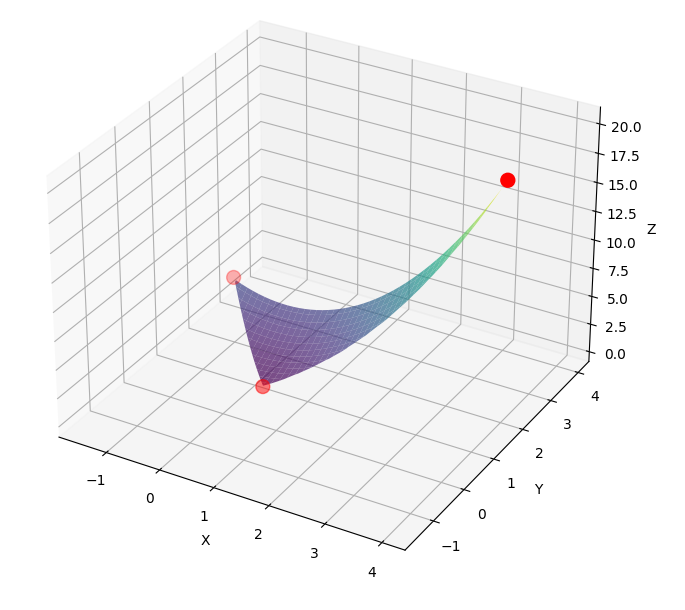
\includegraphics[width=0.5\textwidth]{hyperplane.png}
    \caption{Visualization de $f$ sous les contraintes $c_1, c_2, c_3$}
    \end{figure}
\end{enumerate}

\end{document}
